\subsection{UC3 - Visualizzazione stato dei file}
\begin{figure}[H]
    \centering
    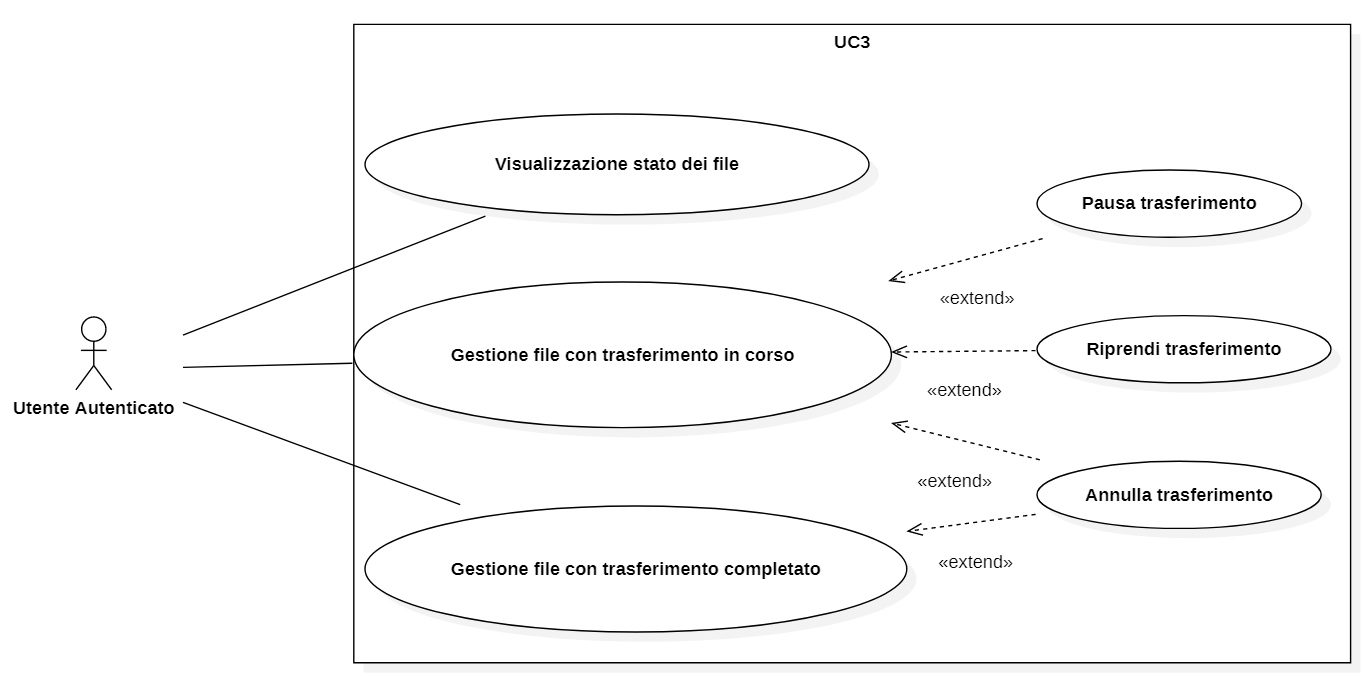
\includegraphics[scale = 0.8]{components/img/UC3.png}
    \caption{UC3 - Visualizzazione stato dei file}
\end{figure}
\begin{itemize}
\item \textbf{Attore Primario:} Utente autenticato;
\item \textbf{Precondizione:} L'utente ha effettuato dei trasferimenti da o verso il server;
\item \textbf{Postcondizione:} L'utente è informato sullo stato dei file sincronizzati e non;
\item \textbf{Scenario principale:}
    \begin{enumerate}
    \item L'utente può visualizzare lo stato corrente dei file.
    \end{enumerate}
\end{itemize}